\documentclass{article}
\usepackage{graphicx}
\usepackage{fullpage}
\title{A short implementation of the exponential function in the C-language}
\author{Camilla Theresia Grøn Sørensen}
\date{}
\begin{document}
\maketitle

\section{About the exponential function}
The exponential function takes an argument $x$ and calculates the Euler's number to the power of the argument.
Euler's number is $e = 2.71828$. The mathematical expression for the exponential function can be seen in equation 
\ref{eq:e}.

\begin{equation}
y = e^x
\label{eq:e}
\end{equation}

\section{Implementing the exponential function in the C-language}
To make it easier for the computer to calculate the value of the exponential function, it is sometimes more useful
to make use the Taylor expansion of the exponential function (equation \ref{eq:Taylor}):

\begin{equation}
y = 1 + x + \frac{x^2}{2!} + \frac{x^3}{3!} + \frac{x^4}{4!} + ... = \Sigma_0^{\infty} x^n
\label{eq:Taylor}
\end{equation}

To make it even easier for the computer to calculate, one can expand equation \ref{eq:Taylor} until you get
equation \ref{eq:expand}:

\begin{equation}
y = 1+x \cdot (1+x/2 \cdot (1+x/3 \cdot (1+x/4 \cdot (1+x/5 \cdot (1+x/6 \cdot(1+x/7 \cdot
(1+x/8 \cdot (1+x/9 \cdot (1+x/10)))))))))
\label{eq:expand}
\end{equation}

It should be noted that equation \ref{eq:expand} is only an approximation to equation \ref{eq:e}.

\section{Test of the implemented exponential function in the C-language}
To test if equation \ref{eq:expand} is a good approximation to equation \ref{eq:e}, both equations are plotted for
$0<x<8$. The result can be seen in figure \ref{fig:exp}.

\begin{figure}
\centering
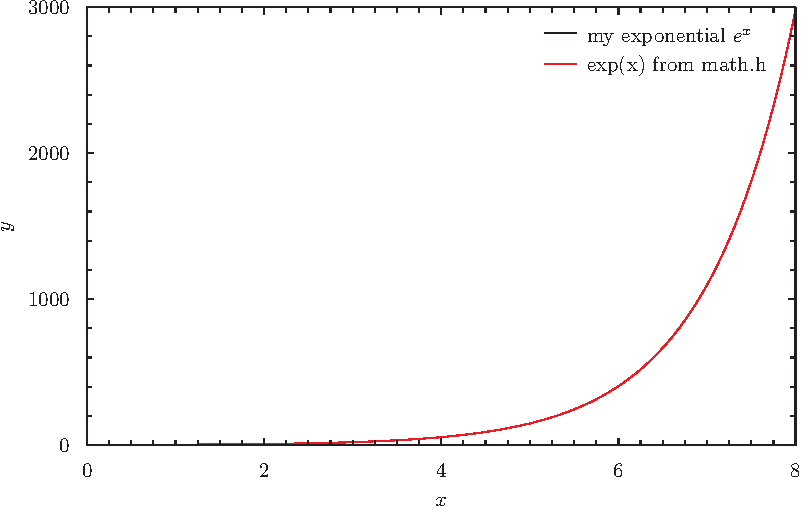
\includegraphics{fig.pdf}
\caption{Plots of equation \ref{eq:expand} (my exponential $e^x$) and equation \ref{eq:e} (exp(x) from math.h).}
\label{fig:exp}
\end{figure}

As it can be seen from figure \ref{fig:exp}, equation \ref{eq:expand} is a good approximation to equation \ref{eq:e}.

\end{document}
